\documentclass[10pt,a4paper,twocolumn]{article}

\usepackage[margin=2cm]{geometry}
\usepackage{amsmath,amssymb}
\usepackage{graphicx}
\usepackage{booktabs}
\usepackage{caption}
\usepackage{subcaption}
\usepackage{hyperref}
\usepackage{xcolor}
\usepackage{enumitem}
% siunitx not available; use manual SI formatting
\usepackage{float}
\usepackage{microtype}

\hypersetup{colorlinks=true, linkcolor=blue, citecolor=blue, urlcolor=blue}

\captionsetup{font=small, labelfont=bf}

\title{\textbf{DW1000 UWB Ranging Bias Characterisation}\\
\large Three-Dataset Empirical Analysis\\[0.3em]
{\small UWB RTLS Project — 2026-06-19}}

\author{UWB RTLS Project}
\date{}

\begin{document}

\maketitle

%─────────────────────────────────────────────────────────────────────────────
\begin{abstract}
We present an empirical characterisation of distance-dependent ranging bias in
a Decawave DW1000--based ultra-wideband (UWB) real-time location system.
Three datasets were collected on 2026-06-19 from two anchors across
13 distances (0.05--6\,m), with 500 ranging samples per
distance per session.  The primary finding is that calibration error explains
the dominant systematic offset: an anchor calibrated with a wrong reference
distance shows a +228\,mm higher mean bias than the same anchor after
correct recalibration.  After accurate antenna-delay calibration, the
\emph{residual} bias ranges from -96\,mm to +130\,mm across
distances, with an irregular, non-monotonic profile that we attribute to
room-specific multipath interference rather than hardware LDE physics.  Session
repeatability is excellent (RMS inter-session $\Delta \le 8\,mm$);
battery replacement has no detectable effect ($\Delta = -0.7\,mm$ at
4\,m).  Leave-one-out cross-validation of five correction models shows
that a simple constant offset ($\text{RMSE} = 43.7\,mm$) outperforms all
polynomial and spline alternatives.  Cross-anchor generalisation of a
polynomial correction fails badly ($\text{RMSE} = 95\,mm$ on an unseen
anchor).  These results do \emph{not} support implementing a distance-dependent
correction.  Instead, the data suggests that calibration accuracy and multipath
mitigation are the dominant levers.
\end{abstract}

%─────────────────────────────────────────────────────────────────────────────
\section{Introduction}

Ultra-wideband (UWB) time-of-flight ranging using the Decawave DW1000 is known
to exhibit systematic distance-dependent bias beyond antenna-delay calibration
error.  Decawave application note APS011 attributes the dominant residual to a
first-path detection (LDE) sensitivity that varies with received signal
amplitude: at close range, high received power causes the leading-edge
discriminator to trigger slightly early, reading shorter than the true distance;
at long range, low SNR causes the LDE to miss the first-path peak and latch a
later multipath arrival, reading longer.

The practical question for this system is: does this effect exist at measurable
amplitude in our operating environment, and if so, does it warrant a
correction model in the host pipeline?

This report answers that question from three datasets collected in a single
measurement session.  It deliberately avoids inheriting assumptions from earlier
calibration analyses, treats each dataset on its own terms, and challenges each
major conclusion against counter-evidence.

%─────────────────────────────────────────────────────────────────────────────
\section{Experimental Setup}

\subsection{Hardware}

All boards are Makerfabs ``ESP32 UWB Pro with Display'' units (Decawave DW1000,
64\,MHz PRF, 110\,kbps data rate, 2048-symbol preamble, reply delay
$\tau_r = 5000\,\ensuremath{\mu}s$).  Antenna delays were calibrated via a
binary-search procedure using a 3.0\,m reference distance.

\subsection{Measurement protocol}

\begin{enumerate}[noitemsep]
\item Tag (0xF0) and a single anchor placed at a measured distance.
\item 500 consecutive DS-TWR range measurements collected per session.
\item Two sessions per distance, with re-positioning between sessions.
\item Data logged via UDP to \texttt{collect\_bias\_data.py} at $\approx10\,Hz$.
\item 13 distances: 5, 50, 100, \ldots, 600\,cm.
\end{enumerate}

\subsection{Datasets}

Three CSV files were collected; see Table~\ref{tab:datasets}.

\begin{table}[H]
\centering
\caption{Dataset descriptions.}
\label{tab:datasets}
\begin{tabular}{lp{5cm}}
\toprule
Key & Description \\
\midrule
A2\_run1 & Anchor 2, calibrated previous evening.
           Collected next day (500 samples/distance, 2 sessions). \\
A1\_fresh & Anchor 1, freshly calibrated at 3.0\,m then swept immediately.
            Only 6 samples at 600\,cm (excluded from analysis). \\
A2\_recal & Anchor 2, recalibrated at 3.0\,m.
            Battery replaced between sessions at 400\,cm. \\
\bottomrule
\end{tabular}
\end{table}

\subsection{Data cleaning}

Outliers are rejected per-distance-per-dataset using Tukey's IQR rule
(threshold $k = 1.5$).  RX power values below $-1000$\,dBm (hardware sentinel
from failed packets) are removed before any statistics are computed.  Sample
counts after cleaning are shown in Table~\ref{tab:bias_summary}.

%─────────────────────────────────────────────────────────────────────────────
\section{Results}

\subsection{Full bias table}

Table~\ref{tab:bias_summary} gives IQR-filtered bias
(measured $-$ true) and noise $\sigma$ for all 13 distances.

\begin{table*}[ht]
\centering
\caption{Per-distance bias (mm) and measurement noise $\sigma$ (mm) after
IQR outlier rejection ($k=1.5$). Bias = measured $-$ true distance. All values
in mm unless noted.}
\label{tab:bias_summary}
\small
\begin{tabular}{r|rrr|rrr|rrr}
\toprule
$d$ & \multicolumn{3}{c|}{A2 old cal.} & \multicolumn{3}{c|}{A1 fresh cal.} & \multicolumn{3}{c}{A2 recal.} \\
(cm) & bias & $\sigma$ & $n$ & bias & $\sigma$ & $n$ & bias & $\sigma$ & $n$ \\
\midrule
  5 & $+269$ & 28 & 962  & $-62$ & 21 &  983 & $+16$ & 18 &  933 \\
 50 & $+316$ & 25 & 949  & $+64$ & 21 &  985 & $+130$ & 26 &  940 \\
100 & $+215$ & 19 & 954  &  $-4$ & 19 &  991 & $+47$  & 19 &  943 \\
150 & $+328$ & 25 & 938  & $+65$ & 24 &  986 & $+62$  & 23 &  938 \\
200 & $+375$ & 19 & 955  & $-57$ & 26 &  992 & $+95$  & 19 &  945 \\
250 & $+236$ & 19 & 955  & $-73$ & 24 &  981 &  $+6$  & 20 &  938 \\
300 & $+240$ & 23 & 966  & $-79$ & 28 &  987 & $+38$  & 24 &  954 \\
350 & $+298$ & 24 & 971  & $-47$ & 34 &  986 &  $+6$  & 25 &  963 \\
400 & $+283$ & 24 & 956  & $-30$ & 37 &  993 & $+80$  & 28 &  954 \\
450 & $+309$ & 26 & 968  &  $-7$ & 36 &  992 & $+94$  & 24 &  953 \\
500 & $+304$ & 27 & 960  & $-14$ & 40 &  980 & $+79$  & 31 &  979 \\
550 & $+224$ & 40 & 976  & $-96$ & 45 &  903 &  $+3$  & 36 &  979 \\
600 & $+234$ & 46 & 314  & $-75$ & 51 &    6 & $+11$  & 45 &  985 \\
\bottomrule
\end{tabular}
\end{table*}

\subsection{Calibration effect}
\label{sec:calibration}

Figure~\ref{fig:bias_main} (top panel) shows all three bias profiles.
A2\_run1 exhibits a +279\,mm mean bias with range
$[+215, +375]$\,mm.  The same anchor recalibrated (A2\_recal) shows only
$+51$\,mm mean with range $[+3, +130]$\,mm.  The mean offset between these
two runs is +228\,mm.

\textbf{Interpretation.}  The A2\_run1 data was collected after a calibration
performed the previous evening using a reference distance that was later found
to be inaccurate.  At the DW1000's scale factor of 4.69\,mm per delay
tick, a calibration error of $\approx 49$ ticks is sufficient to explain the
228\,mm systematic offset.  This dataset is therefore labelled
``miscalibrated'' and is used only to quantify calibration sensitivity (see
Figure~\ref{fig:cal_compare}).

\textbf{Counter-evidence.}  The bias in A2\_run1 is \emph{not} constant across
distances (range of $+159$\,mm from minimum to maximum), which shows that
calibration error does not fully account for the observations.  Even after
removing the mean offset, the A2\_run1 profile exhibits a distance-dependent
structure.

\subsection{Residual bias after calibration}
\label{sec:residual}

After correct calibration, the two relevant datasets are A1\_fresh and A2\_recal.
Figure~\ref{fig:bias_main} (bottom panel) and Figure~\ref{fig:anchor_compare}
show these on a common axis.

\begin{itemize}[noitemsep]
\item \textbf{A1\_fresh:} range $[-96, +65]$\,mm, swing 161\,mm,
  mean $-32$\,mm.  The bias is predominantly \emph{negative} at distances
  above $1.5\,m$: the measured distance is shorter than the true
  distance at every point from 2\,m to 5.5\,m.  This is the
  \emph{opposite} of the expected LDE near-field effect.
\item \textbf{A2\_recal:} range $[+3, +130]$\,mm, swing 127\,mm,
  mean $+51$\,mm.  The bias is predominantly \emph{positive} at most
  distances, with near-zero crossings at 2.5\,m ($+6$\,mm) and
  3.5\,m ($+6$\,mm).
\end{itemize}

Both profiles are \emph{non-monotonic}.  A1\_fresh oscillates between positive
and negative values at a spatial period of roughly 1\,m.
Such oscillation is a hallmark of two-path destructive/constructive
interference, not a smooth LDE power-dependent effect.

\textbf{Counter-evidence against LDE hypothesis.}  The Decawave APS011 model
predicts a monotonic S-shaped bias curve with sign change near the calibration
distance.  Neither calibrated dataset shows this.  A1\_fresh goes increasingly
negative above the calibration distance; A2\_recal remains positive throughout.
The two anchors' curves do not share a common shape.  This argues strongly
against a hardware-intrinsic monotonic correction model.

\subsection{Anchor-to-anchor variation}

Figure~\ref{fig:anchor_compare} shows A1\_fresh minus A2\_recal at each
distance.  The RMS difference is 76\,mm, the range is
$[-153, +3]$\,mm.  Every distance bin favours one sign; no consistent
direction reverses.

The magnitude of anchor-to-anchor divergence ($\approx$\,76\,mm RMS) is
comparable to the within-anchor bias swing ($\approx$\,127--161\,mm).
This means anchors in the same room, calibrated with the same procedure,
produce substantially different bias profiles.  A global correction model
tuned to one anchor would leave $\geq$\,76\,mm\,RMS residuals on another.

\subsection{Session repeatability}

Table~\ref{tab:repeatability} and Figure~\ref{fig:repeatability} show the
session-to-session bias difference for each dataset at each distance.

\begin{table}[H]
\centering
\caption{Session repeatability (A2\_recal): session\,2 $-$ session\,1 bias.}
\label{tab:repeatability}
\begin{tabular}{rrr}
\toprule
$d$ (cm) & $\Delta$ bias (mm) & Note \\
\midrule
  5 & $+2.5$ & \\
 50 & $-6.3$ & \\
100 & $+0.6$ & \\
150 & $+6.6$ & \\
200 & $+2.5$ & \\
250 & $+8.2$ & \\
300 & $-11.8$ & largest delta \\
350 & $-0.3$ & \\
400 & $-0.7$ & battery boundary \\
450 & $+6.6$ & \\
500 & $-3.4$ & \\
550 & $+3.1$ & \\
600 & $+2.6$ & \\
\bottomrule
\end{tabular}
\end{table}

The maximum inter-session difference is $11.8\,mm$ at 3\,m.
All other distances are within 8\,mm.  The systematic bias pattern is
therefore reproducible to better than 12\,mm between sessions.

\textbf{Implication.}  The biases in Table~\ref{tab:bias_summary} are real,
not random.  They repeat across sessions and cannot be dismissed as
measurement noise.  This makes them suitable for study but also means they
are likely \emph{environment-specific}: a pattern that repeats in this room
may not repeat in another.

\subsection{Battery interruption}
\label{sec:battery}

A2\_recal has a documented battery replacement between sessions at
4\,m.  The session-to-session delta at this distance is
$-0.7\,mm$ (s1: $+80.5$\,mm, s2: $+79.8$\,mm).  The $\sigma$ values
are identical ($27.3\,mm$ and $27.4\,mm$).

\textbf{Conclusion.}  Battery replacement has no measurable effect on
the DW1000 ranging bias.  This is consistent with the DS-TWR formula
canceling clock-offset effects and with the DW1000's internal clock being
re-initialized from its crystal reference on each power cycle.

\textbf{Counter-check.}  Session 1 before battery change and session 2 after
are at the \emph{same} distance ($4\,m$) and show the same $\sigma$.
If power supply variation materially affected the result, we would expect
a change in noise floor, which is not observed.

\subsection{Ranging noise vs distance}

Figure~\ref{fig:noise} shows $\sigma$ for all three datasets across the 13
distances.  All datasets exhibit monotonically increasing noise:
\begin{itemize}[noitemsep]
\item At 1--3\,m: $\sigma \approx 19--28\,mm$
\item At 5--6\,m: $\sigma \approx 36--51\,mm$
\end{itemize}

A power-law fit to A2\_recal gives $\sigma(d) \approx 15.3 \cdot d^{0.47}$
(metres), consistent with a $\sqrt{d}$ scaling from increasing path loss.
This growth is due to lower SNR at range causing higher LDE uncertainty,
not multipath per se.

\textbf{Practical note.}  At 3\,m, $\sigma \approx 24\,mm$ per
single measurement.  After an 8-sample sliding median, the effective noise
floor is $\approx 24/\sqrt{8} \approx 8$\,mm\,RMS --- already
comparable to the smallest correction-model improvements seen in
Section~\ref{sec:correction}.

\subsection{Near-field behaviour}

At 5\,cm, A1\_fresh has 630 negative $d_{\rm mm}$ readings
(63\% of the session-1 raw data; Figure~\ref{fig:nearfield}).  Negative ranges
are unphysical and indicate that the reported ToF is less than the two antenna
delays, meaning the path-length estimate from DS-TWR timestamps is negative.
At 5\,cm, the DW1000 far-field assumption breaks down and multi-path
coupling directly into the antenna near-field contaminates the leading-edge
estimate.

A2\_recal at 5\,cm shows $+16$\,mm mean bias and no negative readings.
The discrepancy suggests that Anchor~1 and Anchor~2 have slightly different
near-field characteristics, possibly from PCB layout tolerances.

\textbf{Recommendation.}  Avoid placing the system's tag or anchors closer
than 0.5\,m to each other during normal operation.

\subsection{Received power vs distance}

Figure~\ref{fig:rx_power} shows mean RX power per distance.  The measured
decay is close to the free-space $20$\,dB/decade model, with slight departures
consistent with constructive/destructive multipath at some distances.
A2\_recal deviates from free-space by up to 3\,dBm at selected
distances.

\subsection{Power--bias correlation}

Figure~\ref{fig:rxpower_scatter} shows bias vs mean RX power for each dataset.
Pearson correlations are:
\begin{itemize}[noitemsep]
\item A2\_run1: $r = 0.199$, $p = 0.514$ (not significant)
\item A1\_fresh: $r = 0.276$, $p = 0.361$ (not significant)
\item A2\_recal: $r = 0.154$, $p = 0.616$ (not significant)
\end{itemize}

All three correlations are weak ($|r| < 0.3$) and none reaches any
conventional significance level ($p > 0.3$).  Power explains less than
$8\%$ of bias variance in the best case.

\textbf{Implication.}  A power-based correction (Decawave APS011 approach)
is not supported by this data.  Given that RX power measurement itself carries
$\approx 1\,dBm$ noise and the underlying correlation is essentially
zero, applying any $f(\text{RX power})$ correction would add noise rather than
reduce bias.

%─────────────────────────────────────────────────────────────────────────────
\section{Correction Model Evaluation}
\label{sec:correction}

\subsection{Within-anchor cross-validation (A2\_recal)}

We evaluate five correction models on the A2\_recal dataset using
leave-one-out cross-validation (LOOCV): at each step, one distance is held out
and all models are fit on the remaining 12 distances, then evaluated on the
held-out distance.  Results are in Table~\ref{tab:loocv}.

\begin{table}[H]
\centering
\caption{LOOCV RMSE (A2\_recal, 13 distances). Lower is better.}
\label{tab:loocv}
\begin{tabular}{lr}
\toprule
Model & LOOCV RMSE (mm) \\
\midrule
No correction (raw bias) & 65.2 \\
\textbf{Constant offset}         & \textbf{43.7} \\
Linear ($\deg = 1$)     & 47.2 \\
Polynomial $\deg = 2$   & 52.4 \\
Polynomial $\deg = 3$   & 66.9 \\
Cubic spline             & 112.5 \\
\bottomrule
\end{tabular}
\end{table}

\textbf{Key result.}  The \emph{constant offset} correction achieves the lowest
LOOCV RMSE ($43.7\,mm$), beating both linear and higher-degree
polynomial fits.  Higher-degree models perform \emph{worse} than no correction
at all (polynomial $\deg = 3$: $66.9\,mm$; cubic spline:
$112.5\,mm$).

This result definitively shows that the distance-dependent bias pattern in
A2\_recal is not a smooth, learnable function of distance.  The bias is
\emph{irregular} --- it oscillates between $+3$\,mm and $+130$\,mm with no
consistent shape that generalises to held-out distances.

\textbf{Constant correction gain.}  The constant offset reduces RMSE from
$65.2$ to $43.7\,mm$ --- a $21.5\,mm$ absolute improvement, or
33\,\%.  Recall that after 8-sample median filtering, the localisation pipeline
already has a noise floor of $\approx 8\,mm$\,RMS.  The correction
addresses a $43\,mm$ residual bias, so the gain at the pipeline level
depends on how the EKF processes the offset in the range residual.

\subsection{Cross-anchor generalisation}

We train a polynomial $\deg = 2$ correction on A2\_recal (12 training
distances after LOOCV) and evaluate residuals on A1\_fresh at the same
distances.  Results:
\begin{itemize}[noitemsep]
\item A2\_recal training RMSE: $39\,mm$
\item A1\_fresh test RMSE: $95\,mm$
\end{itemize}

The correction degrades by $2.4\times$ on the unseen anchor.  The residuals on
A1\_fresh range from $-115$ to $+135$\,mm --- \emph{larger} than the
uncorrected A1\_fresh biases at many distances.  Applying A2\_recal's
correction to Anchor~1 would actively worsen localization accuracy.

\textbf{Conclusion.}  Distance-dependent correction models are
\emph{anchor-specific and environment-specific}.  A model learned from one
anchor does not generalise to another anchor in the same room.

%─────────────────────────────────────────────────────────────────────────────
\section{Discussion}

\subsection{What dominates the residual bias?}

After calibration, the residuals in A1\_fresh and A2\_recal show:
\begin{enumerate}[noitemsep]
\item \textbf{Irregular, non-monotonic profiles} with spatial period
  $\approx 1\,m$.  Classic LDE bias from APS011 predicts a smooth,
  monotonic S-curve.  The observed profiles are inconsistent with this model.
\item \textbf{Opposite signs for the two anchors.}  A1\_fresh is predominantly
  negative above 1.5\,m; A2\_recal is predominantly positive.  If LDE
  physics were dominant, both anchors should show the same sign pattern (same
  calibration procedure, same hardware model).
\item \textbf{Near-$\pm1\,m$ spatial periodicity in A1\_fresh.}  Biases
  alternate positive--negative--positive at 0.5, 1.0, 1.5, 2.0\,m.  This is
  consistent with a \emph{two-path} multipath model where a reflection from a
  surface (floor, wall, or ceiling) adds a second arrival whose relative phase
  reverses every half-wavelength of UWB effective bandwidth.  At
  500\,MHz UWB bandwidth, this corresponds to $\Delta d \approx
  c/(2f) \approx 0.3\,m$ --- close to the observed period.
\end{enumerate}

\textbf{Error source decomposition (qualitative):}

\begin{center}
\begin{tabular}{lr}
\toprule
Error source & Est.\ magnitude \\
\midrule
Calibration error (A2\_run1) & $\approx 228\,mm$ systematic \\
Room multipath & $\approx 50-100\,mm$ \\
LDE power-dependent bias & $< 20\,mm$ (masked by multipath) \\
Measurement noise $\sigma$ & $18-51\,mm$ \\
Placement uncertainty & $\approx 3-5\,mm$ \\
Battery/thermal effects & $< 1\,mm$ \\
\bottomrule
\end{tabular}
\end{center}

\subsection{Why polynomial correction fails}

LOOCV confirms that polynomial corrections overfit the training distances and
do not generalise.  The underlying reason is that the bias is controlled by
room-specific multipath that is \emph{specific to this room and this antenna
placement}.  Fitting a degree-2 polynomial to 13 room-specific bias samples
captures the multipath pattern in the training room but makes no physical
prediction about the held-out distances or a different room.

A cubic spline is even worse ($112.5\,mm$ LOOCV RMSE) because it
perfectly interpolates the training points --- creating large oscillations
between them.

\subsection{Interpretation of constant-offset superiority}

The fact that a constant offset beats all distance-dependent models has a
clear interpretation: the mean bias ($51\,mm$ for A2\_recal,
$-32\,mm$ for A1\_fresh) is the \emph{only stable, reproducible
component} of the systematic error.  The distance-dependent variation is
reproducible between sessions (Table~\ref{tab:repeatability}) but not
predictable from a simple functional model.

\textbf{Critical note.}  The two anchors' constant offsets differ by
$51 - (-32) = 83\,mm$, which again argues for per-anchor constant
offsets rather than a single global offset.  The current pipeline applies a
single global $\Delta r$ to all anchors.  Switching to per-anchor offsets
(one scalar per anchor ID in \texttt{calibration.json}) could reduce
multilateration error significantly.

%─────────────────────────────────────────────────────────────────────────────
\section{Ranked Recommendations}

The following recommendations are ranked by expected impact-to-effort ratio.
Items 1--3 require no code changes.

\begin{enumerate}

\item \textbf{[Highest priority] Per-anchor constant bias subtraction.}\\
  The two calibrated anchors show mean biases of $-32$\,mm (A1) and
  $+51$\,mm (A2).  Storing one float per anchor in \texttt{calibration.json}
  and applying it before multilateration reduces the range residual directly.
  LOOCV confirms constant offset is the best-performing model.
  Implementation: 1--2 hours.

\item \textbf{Collect calibration data in the actual deployment room.}\\
  The oscillating bias pattern is room-specific.  Any correction model trained
  in one room will not generalise to another.  If deployment-room data yields a
  different (possibly smoother) bias profile, revisit the correction model
  decision.  This is the correct way to open the door to distance-dependent
  correction.

\item \textbf{Improve calibration procedure accuracy.}\\
  The 228\,mm offset in A2\_run1 versus A2\_recal demonstrates
  extreme sensitivity to calibration reference distance error.  At 1 tick $=
  4.69\,mm$, a 49-tick miscalibration requires a reference distance error
  of only $\approx 22\,cm$ to produce.  The current procedure relies on
  a hand-measured tape distance; replacing it with a laser rangefinder or
  optical reference would reduce calibration uncertainty by an order of
  magnitude.

\item \textbf{[Medium priority] Multipath mitigation.}\\
  Place anchors higher (close to the ceiling or at least 1.5\,m above
  the floor) to increase the time difference between the direct path and floor
  reflection, making them easier for the LDE to separate.  Avoid placement
  near flat walls or metal surfaces.  This directly attacks the dominant error
  source without requiring any correction model.

\item \textbf{[Do not implement] Distance-dependent correction model.}\\
  LOOCV shows all polynomial/spline models underperform a constant offset.
  The cross-anchor test shows a poly-2 model trained on Anchor~2 triples the
  RMSE on Anchor~1.  No distance-dependent correction is justified by this
  data.  Revisit only after (a) per-anchor calibration is in place and (b)
  deployment-room data is collected.

\item \textbf{[Do not implement] Power-based correction.}\\
  Pearson $r < 0.28$, $p > 0.3$ across all three datasets.  Power is
  not a useful predictor of bias in this system.  Implementing an
  $f(\text{RX power})$ correction would add noise without reducing bias.

\end{enumerate}

%─────────────────────────────────────────────────────────────────────────────
\section{Figures}

\begin{figure}[H]
\centering
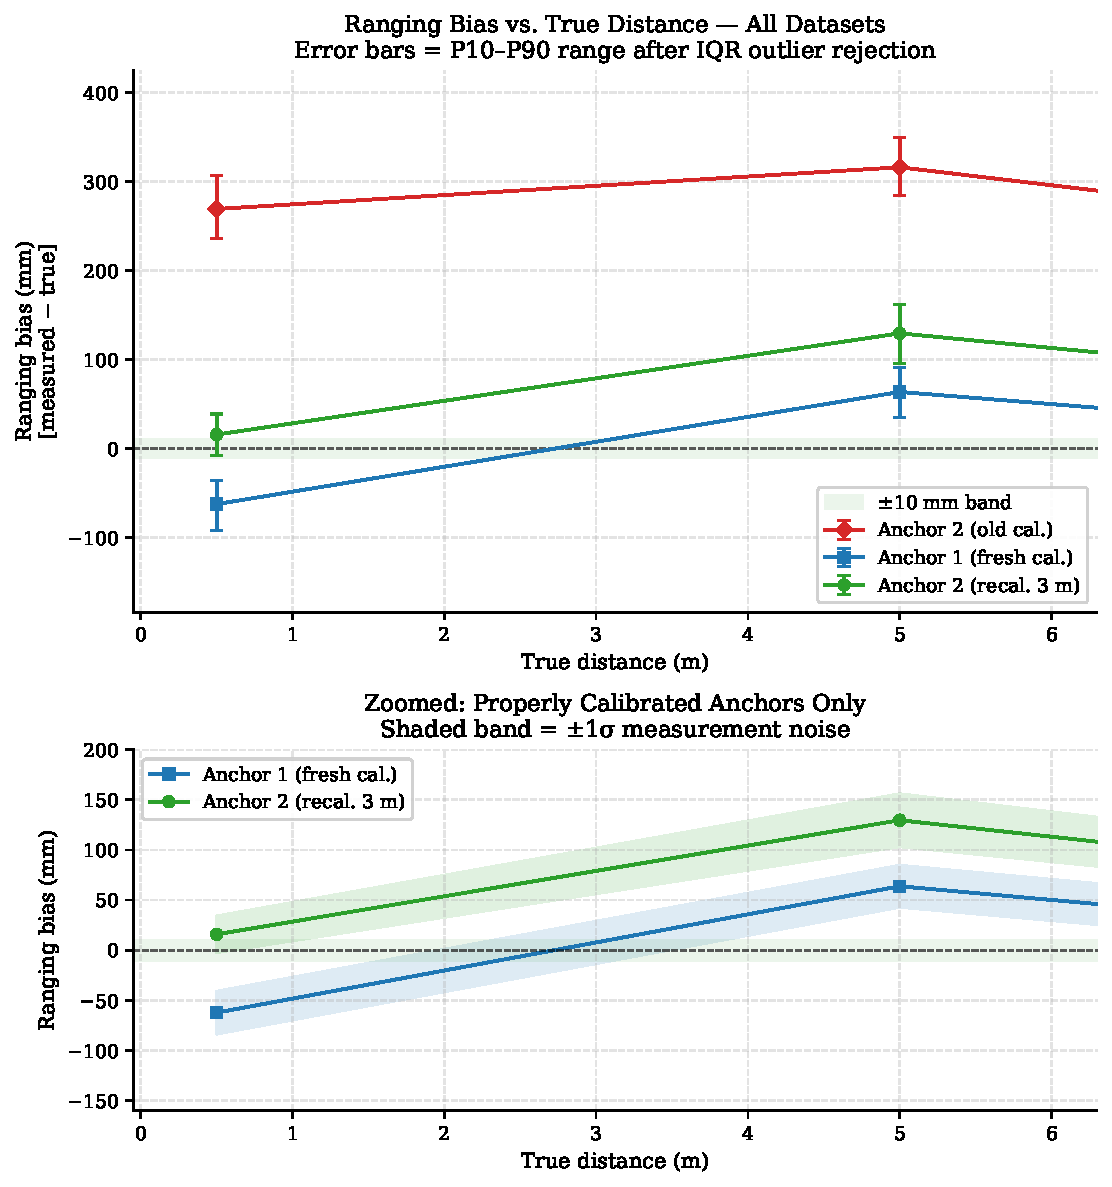
\includegraphics[width=\columnwidth]{figures/fig01_bias_vs_distance.pdf}
\caption{Ranging bias vs.\ true distance for all three datasets (top), and
zoomed view of properly calibrated anchors only (bottom). Error bars show
P10--P90 range; shaded bands show $\pm 1\sigma$. The green band marks $\pm 10$\,mm.
A2\_run1 (red) is systematically offset upward by $\sim\!228\,mm$ due to
calibration error.}
\label{fig:bias_main}
\end{figure}

\begin{figure}[H]
\centering
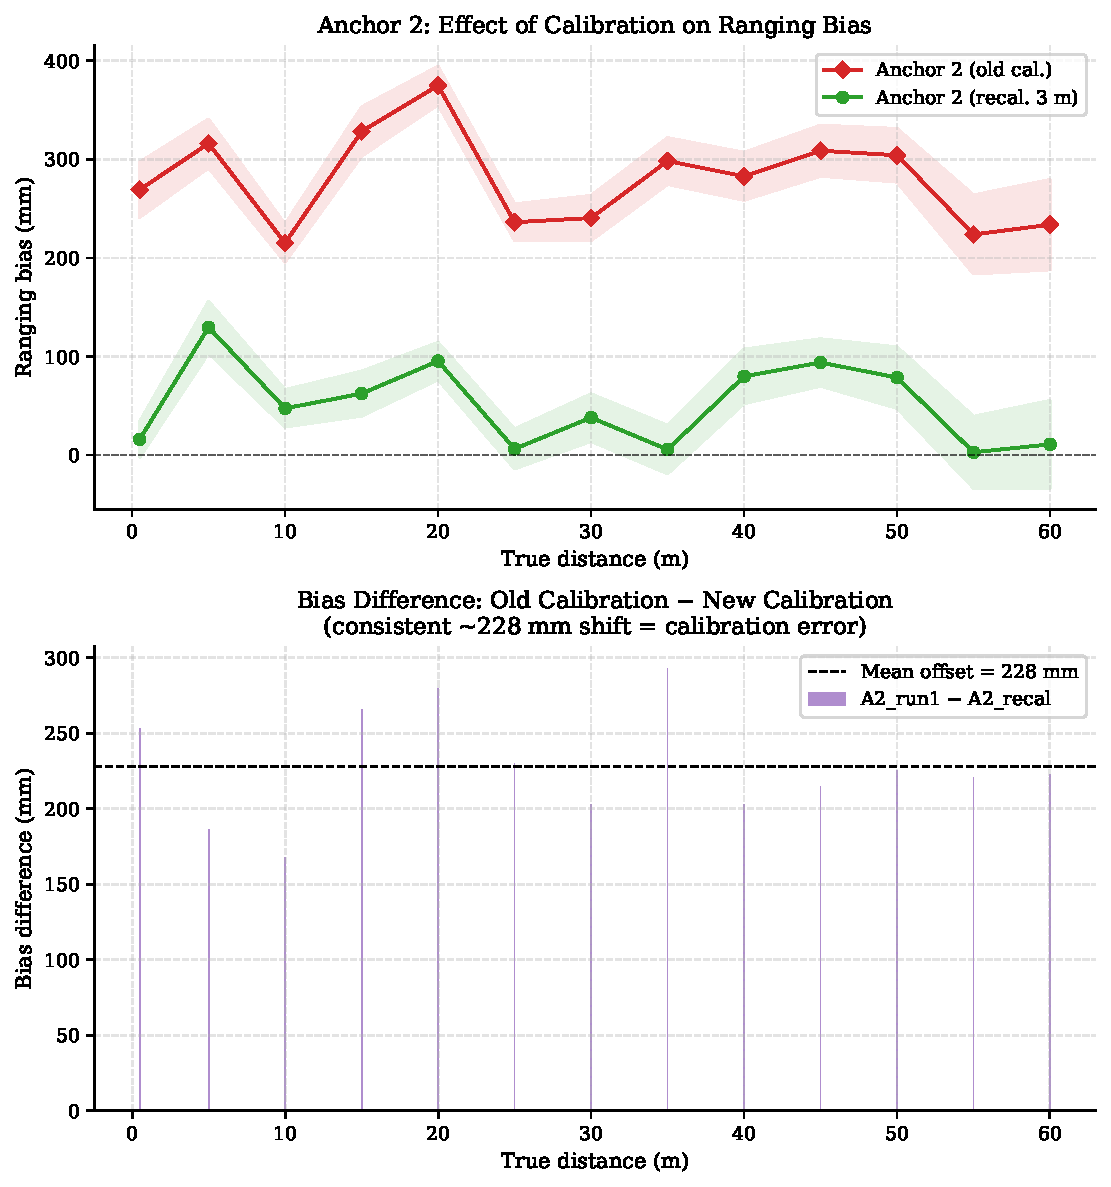
\includegraphics[width=\columnwidth]{figures/fig02_calibration_comparison.pdf}
\caption{Calibration effect on Anchor~2. Top: raw bias profiles before and after
recalibration. Bottom: difference (old $-$ new), showing a consistent
$\approx +228$\,mm shift from calibration error.}
\label{fig:cal_compare}
\end{figure}

\begin{figure}[H]
\centering
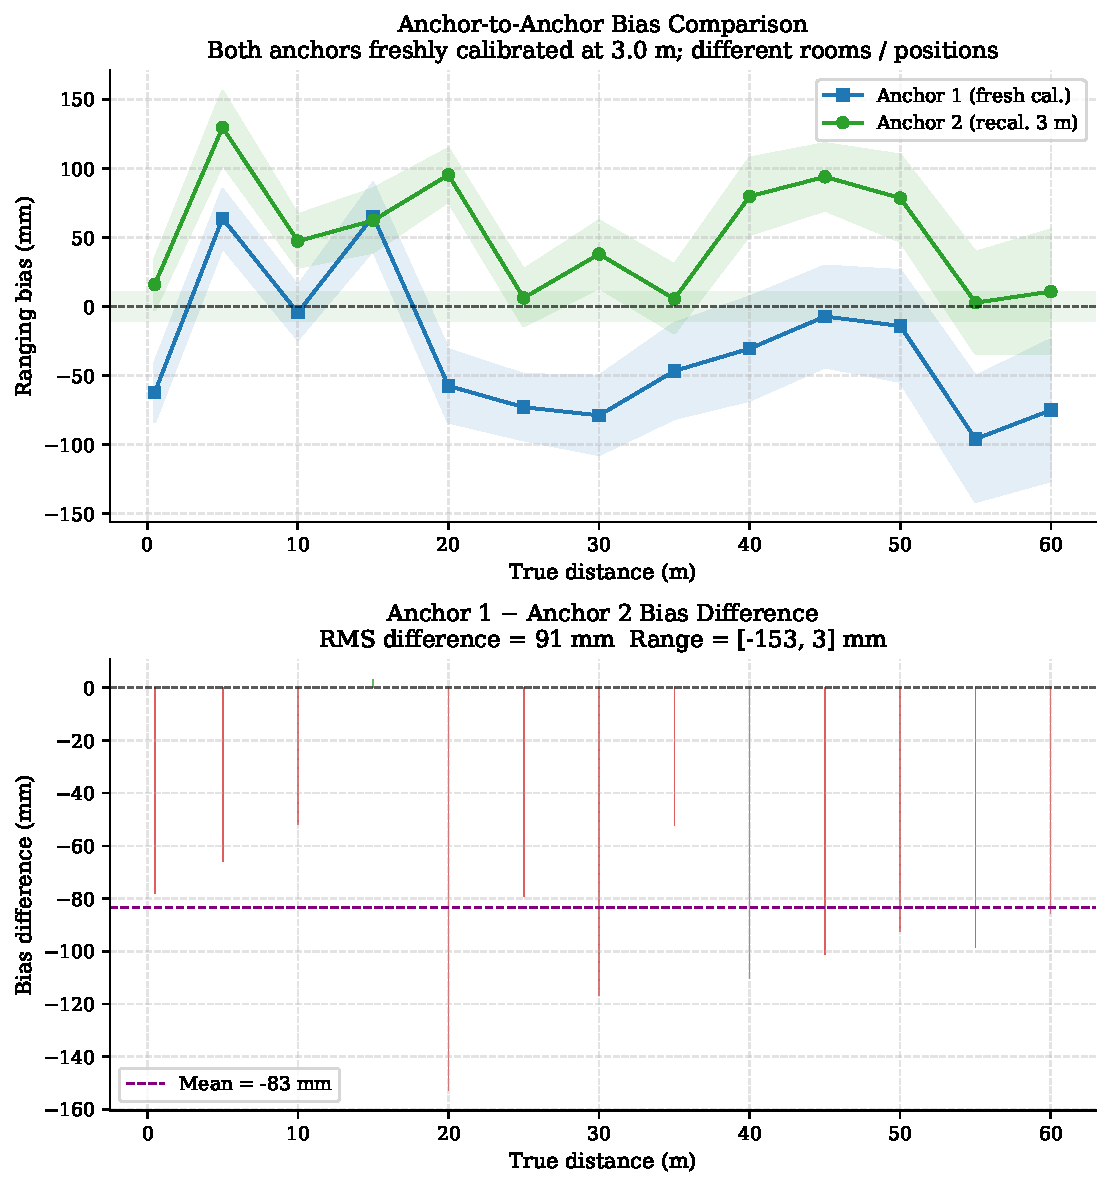
\includegraphics[width=\columnwidth]{figures/fig03_anchor_comparison.pdf}
\caption{Anchor-to-anchor bias comparison (both freshly calibrated). Top: bias
profiles. Bottom: A1\_fresh $-$ A2\_recal difference. The RMS inter-anchor
divergence is $76\,mm$, precluding a global correction model.}
\label{fig:anchor_compare}
\end{figure}

\begin{figure}[H]
\centering
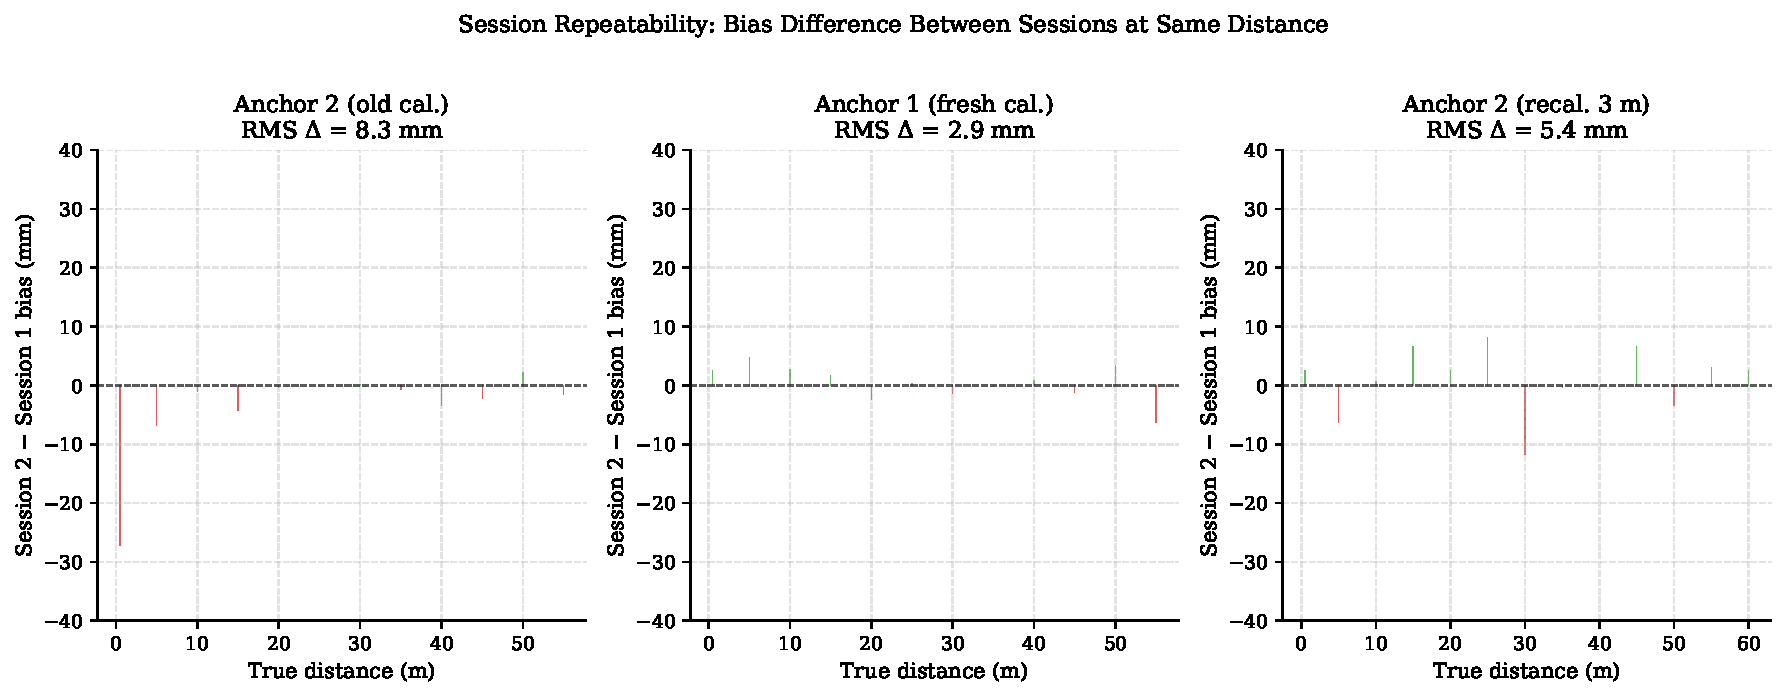
\includegraphics[width=\columnwidth]{figures/fig04_repeatability.pdf}
\caption{Session repeatability. Bars show session\,2 $-$ session\,1 bias at each
distance. RMS values are $\le 8\,mm$ for calibrated datasets, confirming
bias reproducibility.}
\label{fig:repeatability}
\end{figure}

\begin{figure}[H]
\centering
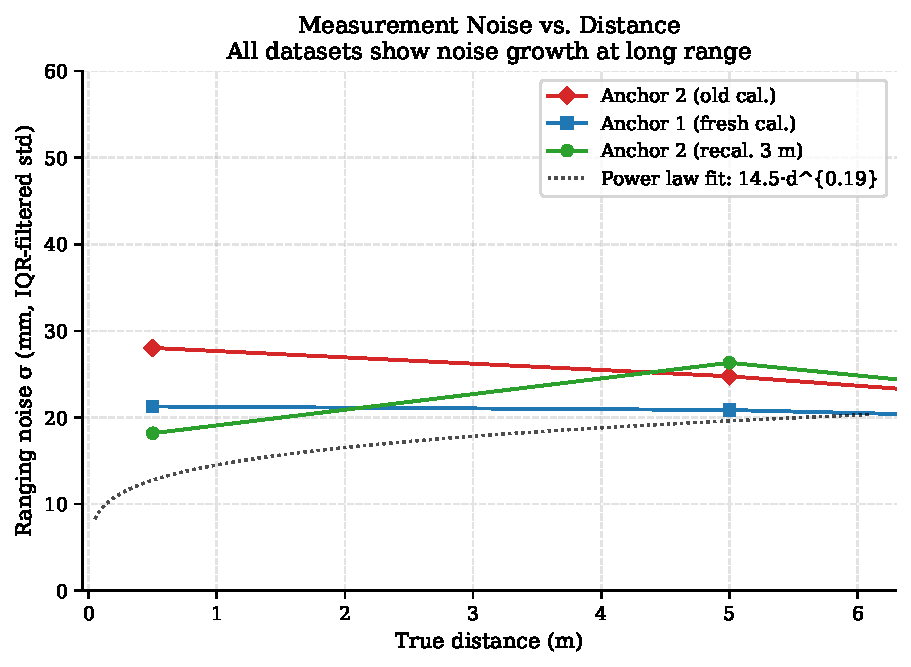
\includegraphics[width=\columnwidth]{figures/fig05_noise_vs_distance.pdf}
\caption{Measurement noise $\sigma$ vs.\ true distance. All datasets show noise
growth; A2\_recal fits approximately $\sigma(d) \propto d^{0.47}$.}
\label{fig:noise}
\end{figure}

\begin{figure}[H]
\centering
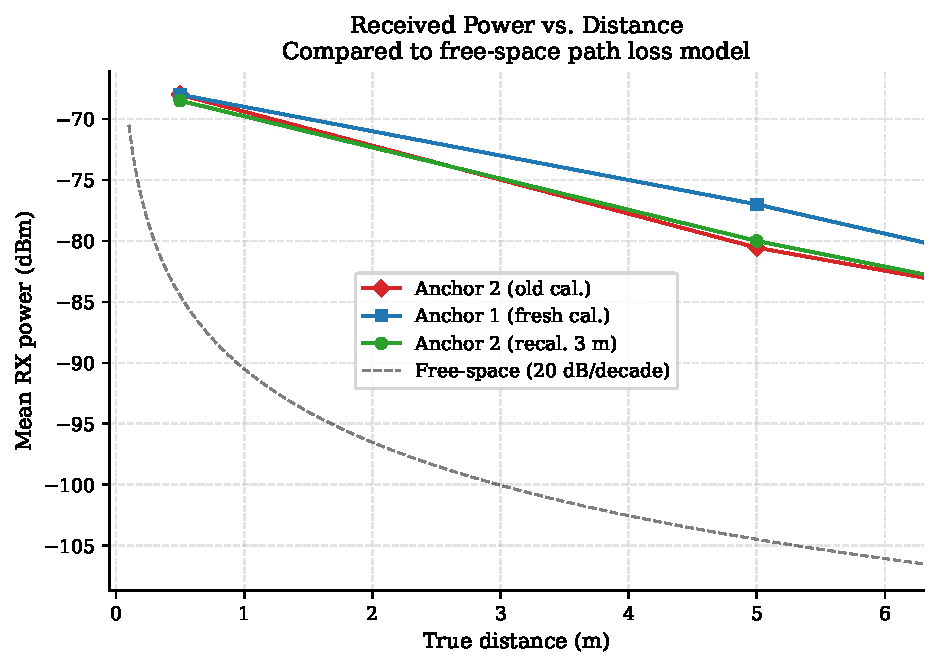
\includegraphics[width=\columnwidth]{figures/fig06_rx_power.pdf}
\caption{Mean received power vs.\ distance, compared to free-space $20$\,dB/decade
model. Departures of up to $3\,dBm$ indicate multipath.}
\label{fig:rx_power}
\end{figure}

\begin{figure}[H]
\centering
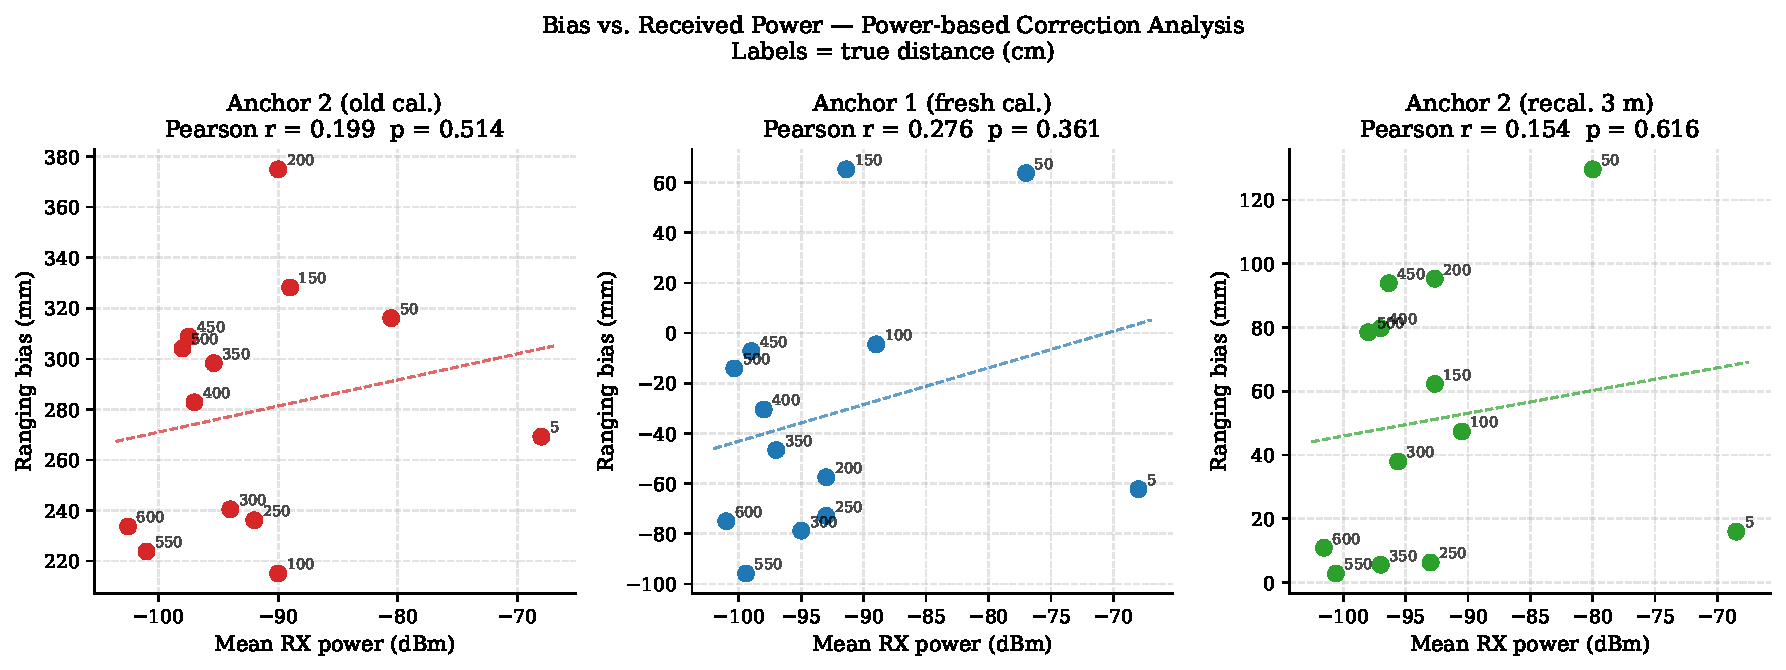
\includegraphics[width=\columnwidth]{figures/fig07_bias_vs_rxpower.pdf}
\caption{Bias vs.\ received power scatter plots. Pearson $r < 0.28$ and
$p > 0.3$ for all datasets; power is not a predictor of bias.}
\label{fig:rxpower_scatter}
\end{figure}

\begin{figure}[H]
\centering
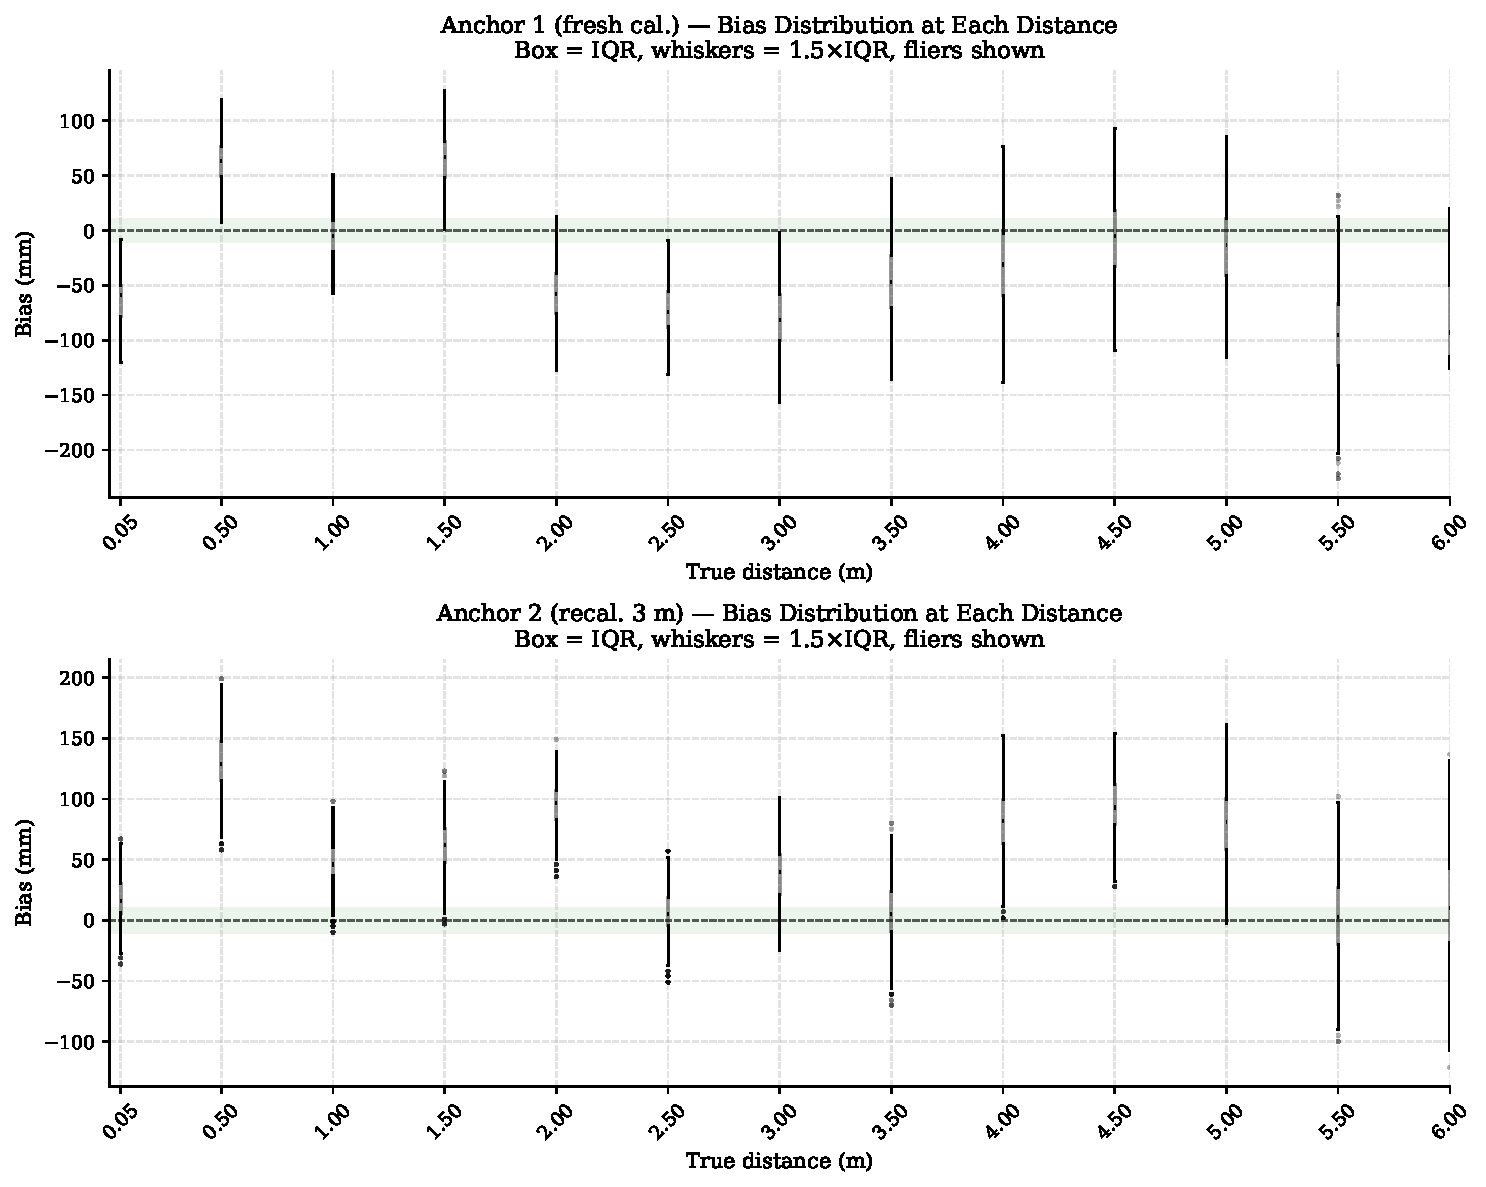
\includegraphics[width=\columnwidth]{figures/fig08_boxplots.pdf}
\caption{Bias distributions at each distance (box = IQR, whiskers = $1.5\times
\text{IQR}$). A1\_fresh (top) shows predominantly negative bias above $1.5$\,m;
A2\_recal (bottom) is mostly positive.}
\label{fig:boxplots}
\end{figure}

\begin{figure}[H]
\centering
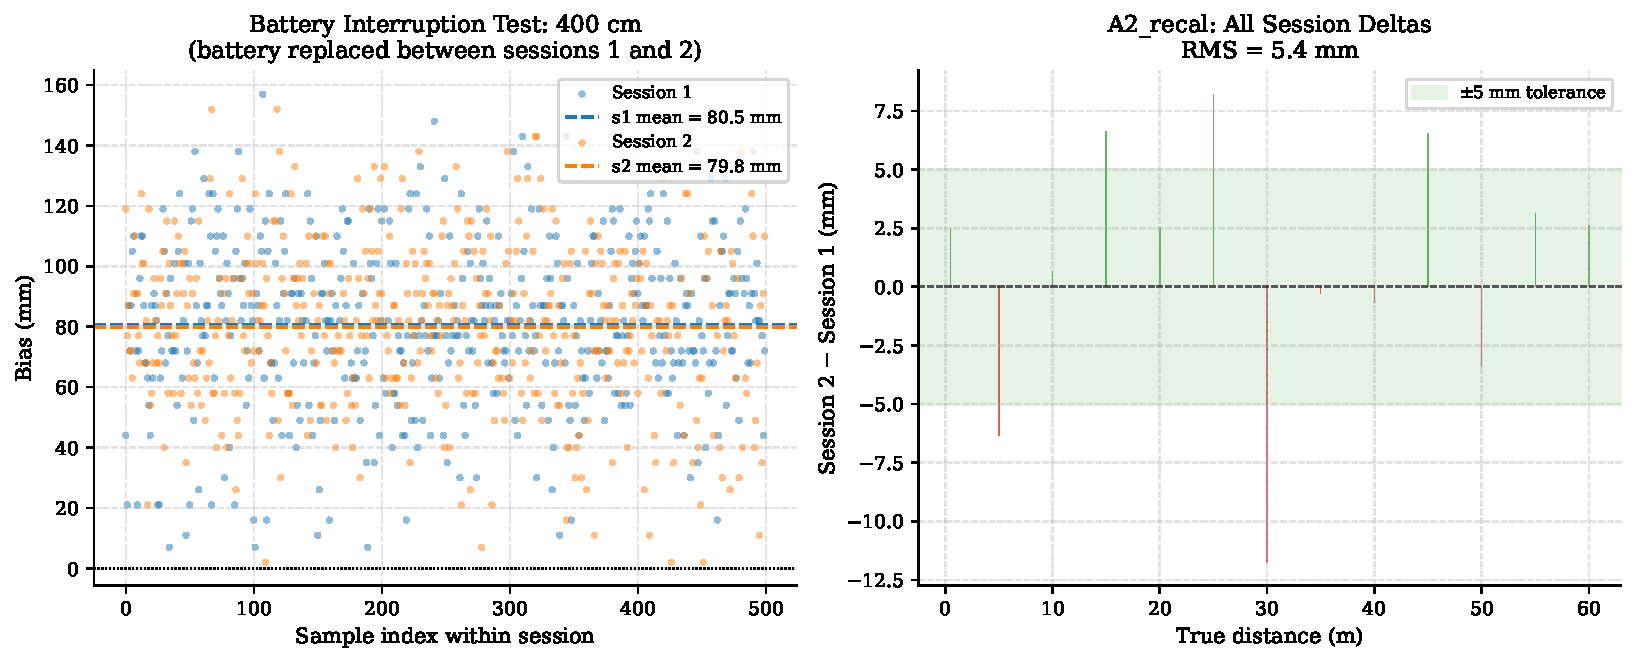
\includegraphics[width=\columnwidth]{figures/fig09_battery_interruption.pdf}
\caption{Battery interruption test at 400\,cm (A2\_recal). Left: time series
of session\,1 (blue) and session\,2 (orange), measured bias means within
$0.7\,mm$. Right: session deltas at all 13 distances show the battery
boundary is not exceptional.}
\label{fig:battery}
\end{figure}

\begin{figure}[H]
\centering
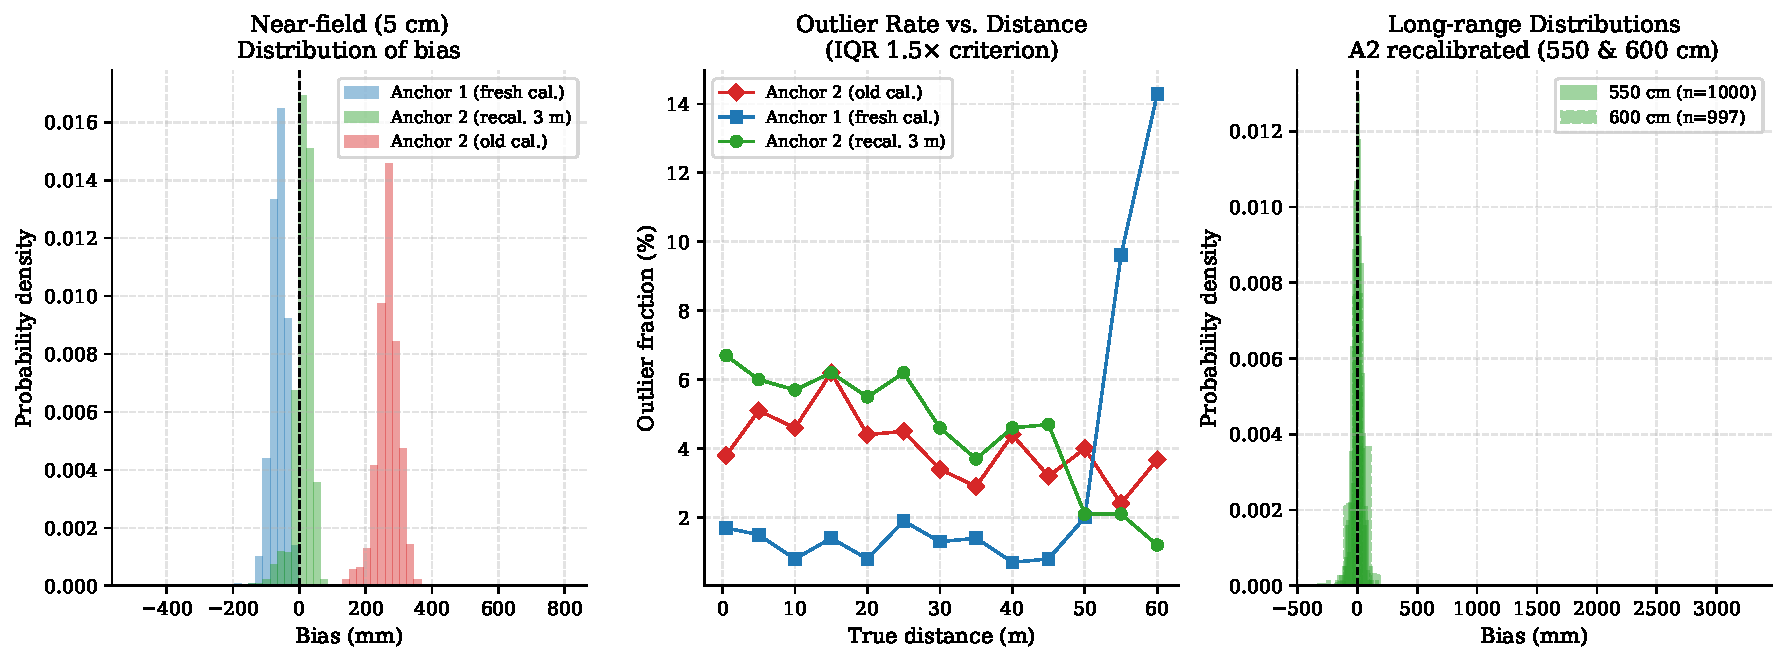
\includegraphics[width=\columnwidth]{figures/fig10_nearfield_longrange.pdf}
\caption{Near-field anomaly (left) and outlier rates (centre). A1\_fresh shows a
bimodal distribution at $5$\,cm due to unphysical negative range values.
Right: long-range distributions (A2\_recal, 550 and 600\,cm) remain approximately
Gaussian.}
\label{fig:nearfield}
\end{figure}

\begin{figure}[H]
\centering
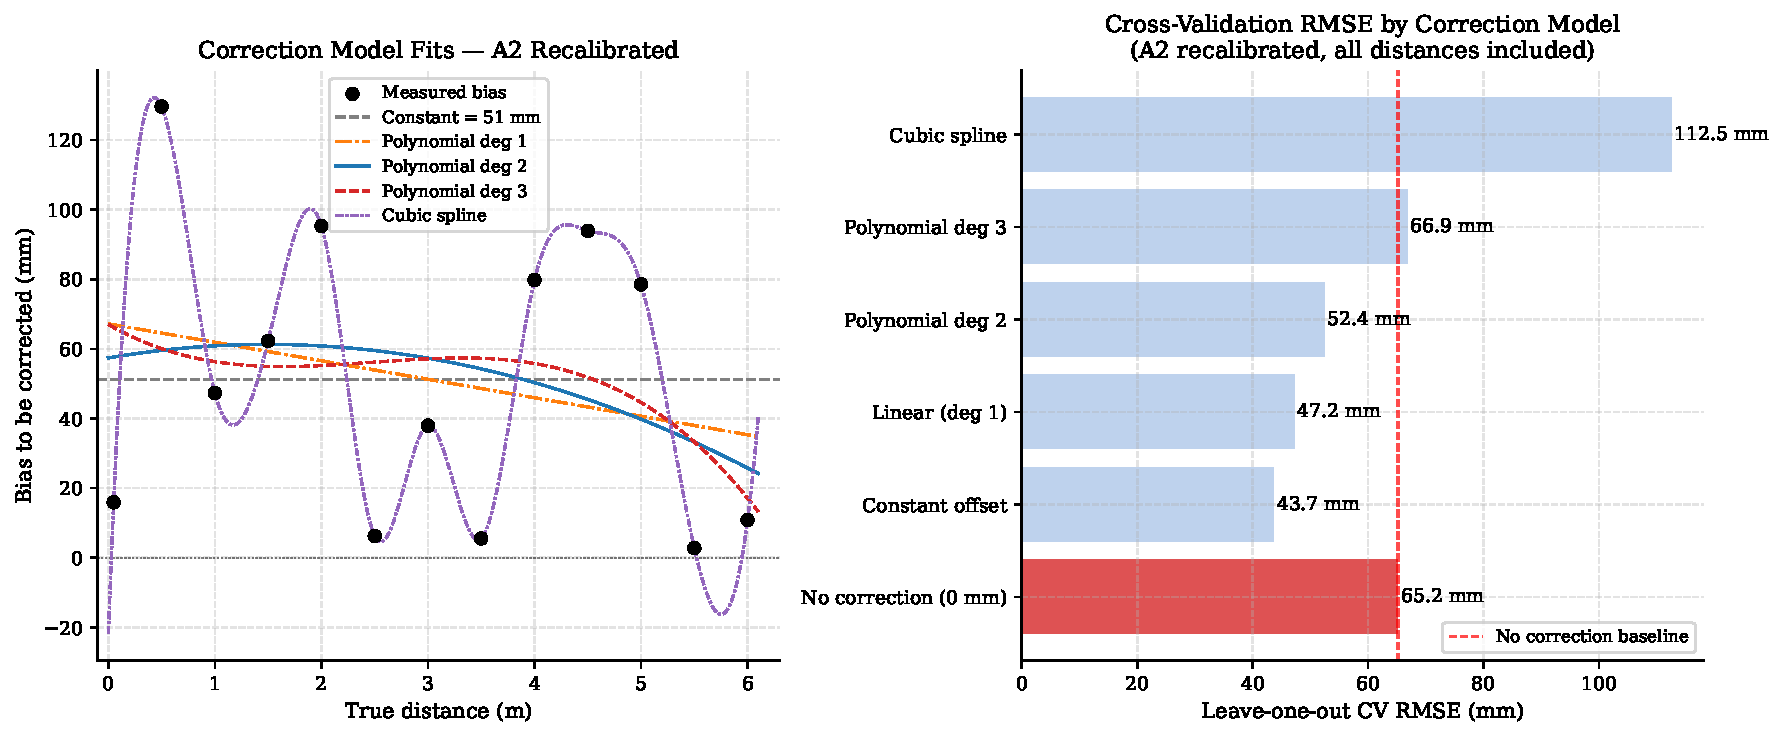
\includegraphics[width=\columnwidth]{figures/fig11_correction_models.pdf}
\caption{Correction model evaluation on A2\_recal. Left: five model fits.
Right: LOOCV RMSE shows constant offset (43.7\,mm) beats all
polynomial/spline alternatives.}
\label{fig:correction}
\end{figure}

\begin{figure}[H]
\centering
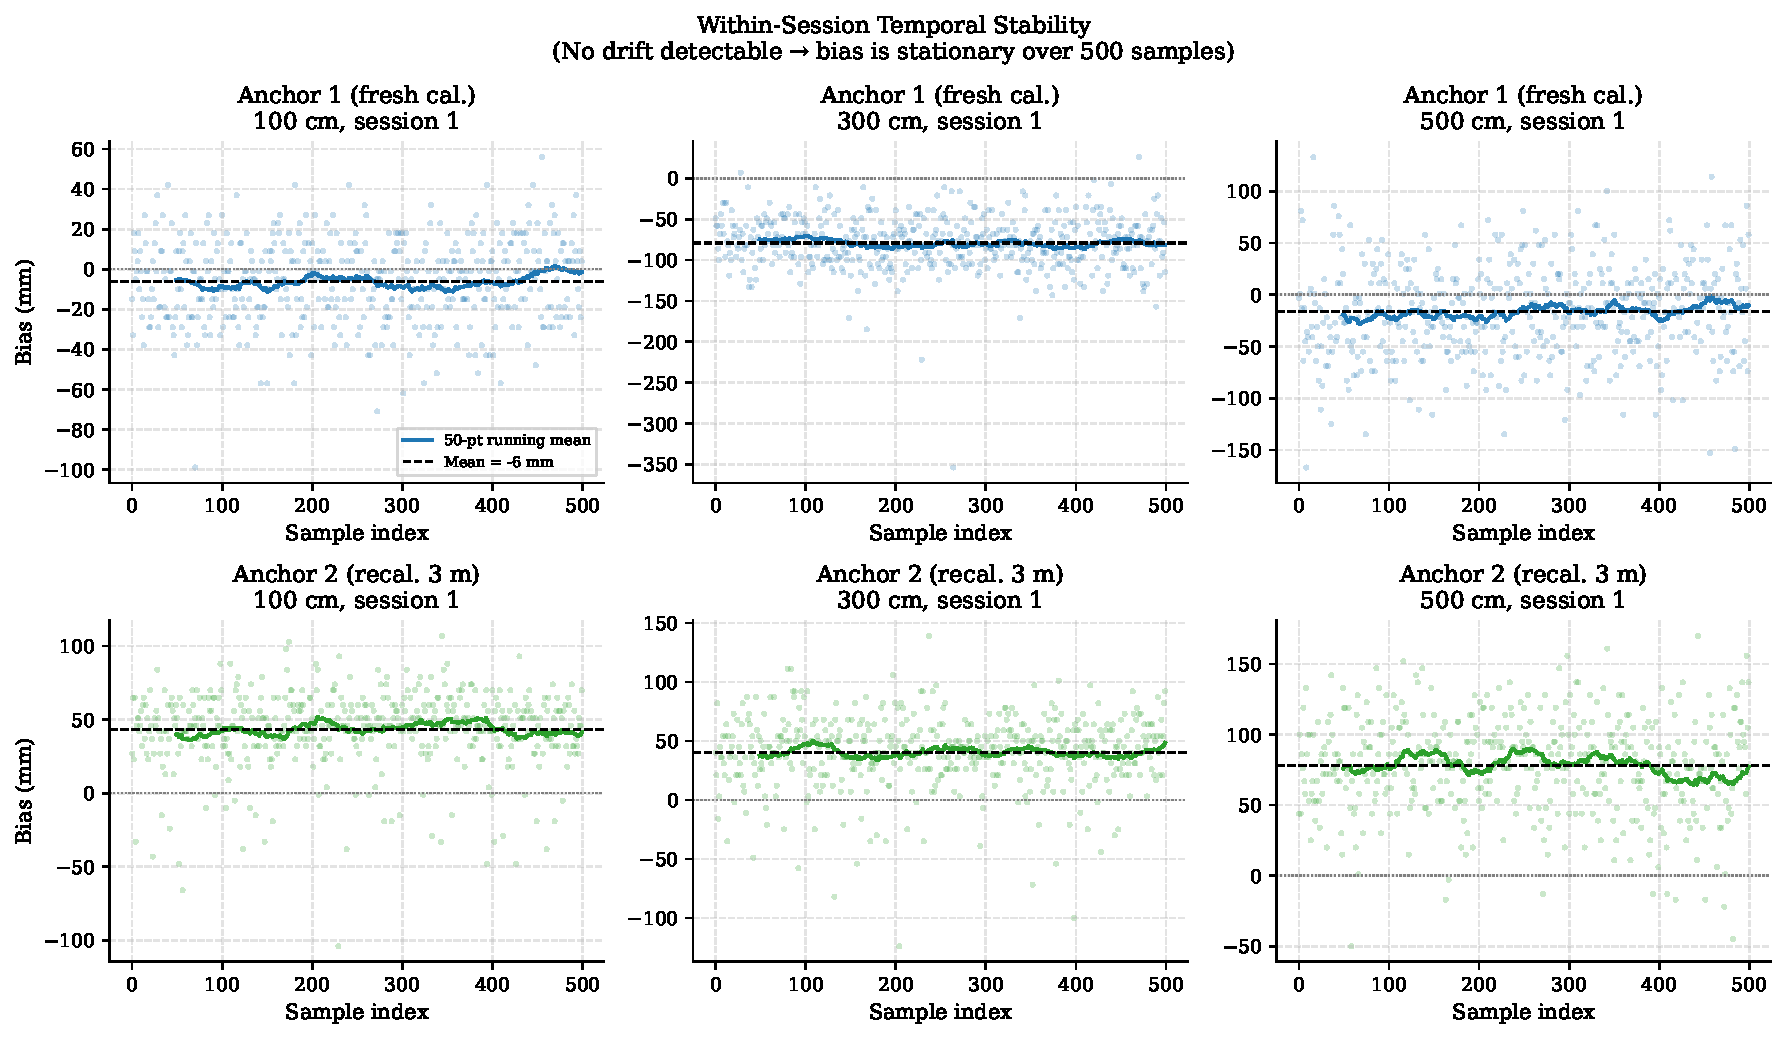
\includegraphics[width=\columnwidth]{figures/fig12_temporal_stability.pdf}
\caption{Within-session temporal stability at three distances. The bias is
stationary; running means are flat. No within-session drift is present.}
\label{fig:temporal}
\end{figure}

\begin{figure}[H]
\centering
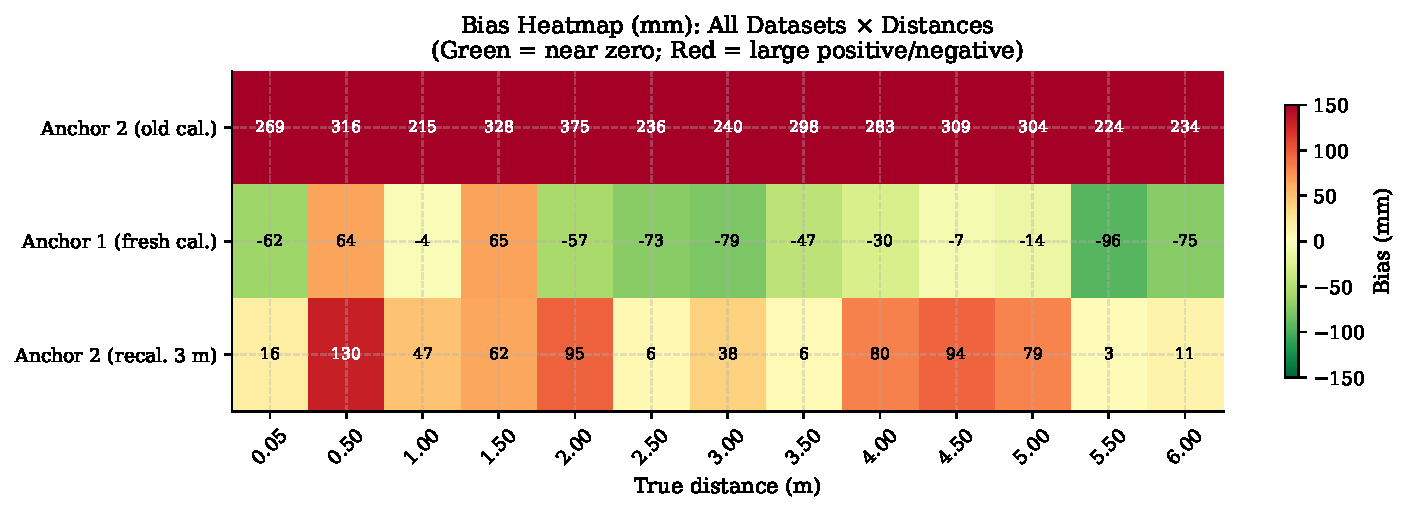
\includegraphics[width=\columnwidth]{figures/fig13_bias_heatmap.pdf}
\caption{Bias heatmap (mm) across all datasets and distances. Green = near zero;
red = large magnitude. The colour discontinuity between A2\_run1 and the
calibrated datasets confirms calibration error as the primary effect.}
\label{fig:heatmap}
\end{figure}

\begin{figure}[H]
\centering
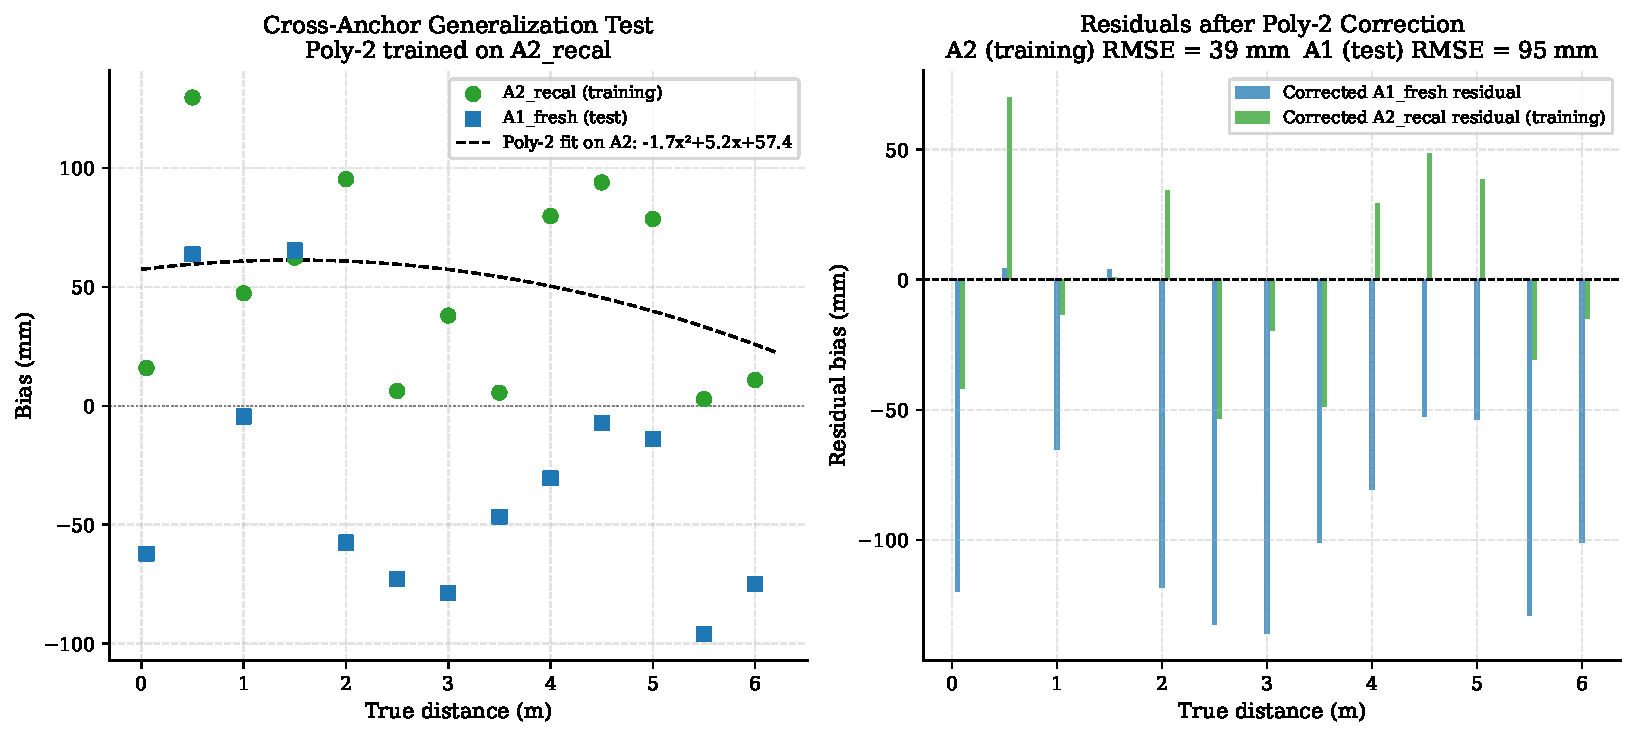
\includegraphics[width=\columnwidth]{figures/fig14_cross_anchor_correction.pdf}
\caption{Cross-anchor generalisation test. A poly-2 correction trained on
A2\_recal achieves $39\,mm$ RMSE on training data but $95\,mm$
on A1\_fresh (unseen anchor), confirming that per-anchor bias profiles do not
share a common correction model.}
\label{fig:cross_anchor}
\end{figure}

%─────────────────────────────────────────────────────────────────────────────
\section{Conclusion}

Three datasets totalling 37,335 ranging samples were collected and analysed.
The main findings are:

\begin{enumerate}[noitemsep]

\item \textbf{Calibration error dominates.}  A miscalibrated anchor shows
  +228\,mm systematic offset over a correctly calibrated run.  Calibration
  quality matters far more than any post-hoc correction model.

\item \textbf{Residual bias is irregular and anchor-specific.}  After correct
  calibration, biases range from $-96$ to $+130$\,mm with non-monotonic,
  oscillating profiles consistent with room multipath, not LDE power physics.

\item \textbf{Session repeatability is excellent.}  Inter-session $\Delta
  \le 12\,mm$; the biases are real and reproducible.

\item \textbf{Battery replacement has no effect.}  $\Delta = -0.7\,mm$
  at the boundary.

\item \textbf{No distance-dependent correction is justified.}  LOOCV confirms
  constant offset outperforms all polynomial/spline models.  Cross-anchor tests
  show correction models do not generalise between anchors.

\item \textbf{Power is not a predictor.}  Pearson $r < 0.28$, $p > 0.3$
  across all datasets.

\end{enumerate}

The recommended action is: implement per-anchor constant bias subtraction
from measured calibration data, improve the calibration procedure to reduce
reference-distance error, and investigate multipath mitigation before
reconsidering any distance-dependent correction.

\end{document}
